\documentclass[12pt]{report}

\usepackage{hcmus-report-template}

% Disable indentation on new paragraphs
\setlength{\parindent}{0pt}

% Line spacing 1.5
\renewcommand{\baselinestretch}{1.5}

% Optional: graphic path
% \graphicspath{PATH_TO_GRAPHIC_FOLDER}

% To use Times font family, uncomment this row
% \usepackage{mathptmx}

% To use roman section / subsection, uncomment these rows
% \renewcommand{\thesection}{\Roman{section}}
% \renewcommand{\thesubsection}{\thesection.\Roman{subsection}}

% Define course name, report name and report title.
\newcommand{\coursename}{Tư duy tính toán}
\newcommand{\reportname}{TourXport - Smart Tourism System}
\newcommand{\reporttitle}{Proof of Concept}

\newcommand{\studentname}{Phạm Anh Tuấn - 24120238 \\ Nguyễn Anh Đức - 24120289 \\ Nguyễn Đức Anh Khôi - 24120076 \\ Võ Minh Khang - 24120336 \\ Nguyễn Quốc Nam - 24120098 \\ Phan Văn Việt - 24120244 \\ Nguyễn Anh Thái - 24120224}
\newcommand{\teachername}{ThS. Nguyễn Trọng Việt}

% Header
\lhead{\reporttitle}
\rhead{
Trường Đại học Khoa học Tự nhiên - ĐHQG HCM\\
\coursename
}

% Footer
% Customize the footer text if desired. Leaving it empty hides the footer.
\newcommand{\leftfooter}{}
\lfoot{\leftfooter}
\usepackage{titlesec}

% Tùy chỉnh khoảng cách cho Chương
% \titlespacing*{loại_tiêu_đề}{thụt_lề_trái}{khoảng_cách_trên}{khoảng_cách_dưới}
\titleformat{\chapter}[hang]{\bfseries\Large}{CHƯƠNG \thechapter:}{0.5em}{}
\titlespacing*{\chapter}{0pt}{-30pt}{20pt} 

% Tùy chỉnh thêm cho các Section nếu thấy nó cũng quá thưa
\titlespacing*{\section}{0pt}{12pt}{6pt}

\usepackage{titlesec}
\usepackage{etoolbox}
\usepackage{array}
\usepackage{titletoc}
\usepackage{xcolor}

% 1. Đảm bảo hyperref nhận màu xanh cho cả cụm (nếu chưa có)
\hypersetup{colorlinks=true, linkcolor=blue}

% 2. Cấu hình lại Mục lục
\titlecontents{chapter}
    [0pt]                               % Lề trái
    {\addvspace{10pt}\bfseries\color{blue}} % Đổi màu cả dòng Chương thành màu xanh
    {CHƯƠNG \thecontentslabel:\hspace{0.5em}} % Giảm khoảng cách sau dấu ":" bằng \hspace
    {}                                  
    {\hfill\contentspage}

% 3. Giảm khoảng cách cho Section (mấy số 1, 2, 3 xanh xanh)
\titlecontents{section}
    [1.5em]                             % Thụt lề trái cho Section
    {\addvspace{3pt}\color{blue}}       % Giữ màu xanh
    {\thecontentslabel\hspace{0.5em}}   % Giảm khoảng cách giữa số "1" và tiêu đề
    {}
    {\titlerule*[0.8pc]{.}\contentspage}

% 4. Tương tự cho Subsection nếu cần
\titlecontents{subsection}
    [3.8em]
    {\addvspace{1pt}\color{blue}}
    {\thecontentslabel\hspace{0.5em}}
    {}
    {\titlerule*[0.8pc]{.}\contentspage}

% Giữ nguyên các định dạng đè số nãy giờ của ông
\renewcommand{\thesection}{\arabic{section}}
\renewcommand{\thesubsection}{\thesection.\arabic{subsection}}
\renewcommand{\thesubsubsection}{\thesubsection.\arabic{subsubsection}}

% 2. Reset số Section mỗi khi bắt đầu Chương mới
\makeatletter
\@addtoreset{section}{chapter}
\makeatother

% 3. Định nghĩa lại cách hiển thị số cho Section, Subsection, Subsubsection
\renewcommand{\thesection}{\arabic{section}}
\renewcommand{\thesubsection}{\thesection.\arabic{subsection}}
\renewcommand{\thesubsubsection}{\thesubsection.\arabic{subsubsection}}

% 4. Ép Subsubsection hiện lên trên Mục lục (Table of Contents)
\setcounter{tocdepth}{3}    % Hiện đến cấp 3 (Subsubsection)
\setcounter{secnumdepth}{3} % Đánh số đến cấp 3
% 5. Tùy chỉnh nốt cho Subsubsection (Cấp 1.1.1)
\titlecontents{subsubsection}
    [6.5em]                             % Thụt lề trái (tăng lên để không đè lên subsection)
    {\addvspace{1pt}\color{blue}}       % Vẫn màu xanh cho đồng bộ
    {\thecontentslabel\hspace{0.5em}}   % Giảm khoảng cách số 1.1.1 với tiêu đề
    {}
    {\titlerule*[0.8pc]{.}\contentspage}
% ============ DOCUMENT ============
\begin{document}

\pagenumbering{roman}
\begin{titlepage}
\newcommand{\HRule}{\rule{\linewidth}{0.3mm}}
\centering

\textsc{\LARGE đại học quốc gia tphcm}\\[0.3cm]
\textsc{\Large trường đại học khoa học tự nhiên}\\[0.3cm]
\textsc{\large khoa công nghệ thông tin}\\[0.3cm]
% \textsc{bộ môn phương pháp lập trình hướng đối tượng}\\[0.5cm]

\HRule \\[0.3cm]
{ 
\huge{\bfseries{\reporttitle}}\\[0.3cm]
}
\HRule \\[0.3cm]

\textbf{\large Môn học: \coursename}\\[0.3cm]

\begin{minipage}[t]{0.45\textwidth}
\begin{flushleft} \large
\emph{Sinh viên thực hiện:}\\
\studentname
\end{flushleft}
\end{minipage}
% \hfill
\begin{minipage}[t]{0.45\textwidth}
\begin{flushright} \large
\emph{Giáo viên hướng dẫn:} \\
\teachername
\end{flushright}
\end{minipage}\\[0.3cm]

{\large \today}\\[0.3cm]


\includegraphics[scale=.3]{img/hcmus-logo.png}\\[1cm] 

\vfill
\end{titlepage}
	


\section*{Danh sách thành viên}

\begin{table}[H]
\centering
\renewcommand{\arraystretch}{1.3}
\begin{tabular}{|c|m{4.5cm}|m{4cm}|m{6cm}|}
\hline
\textbf{MSSV} & \multicolumn{1}{c|}{\textbf{Họ và tên}} & \multicolumn{1}{c|}{\textbf{Vai trò}} & \multicolumn{1}{c|}{\textbf{Nhiệm vụ}} \\ \hline
24120238 & Phạm Anh Tuấn & Frontend developer \newline Project Manager & Thiết kế giao diện và phát triển app Flutter. \newline Quản lý tiến độ dự án. \newline Viết báo cáo Chương 1. \\ \hline
24120289 & Nguyễn Anh Đức & Frontend developer & Thiết kế giao diện và phát triển app Flutter. \newline Viết báo cáo phần 2 Chương 3. \\ \hline
24120098 & Nguyễn Quốc Nam & Backend developer \newline DevOps Engineer & Thiết kế và phát triển Backend. \newline Cấu hình môi trường, Docker và triển khai hệ thống lên Server. \newline Tổng hợp báo cáo\\ \hline
24120244 & Phan Văn Việt & Backend developer & Thiết kế và phát triển Backend. \newline Viết báo cáo Chương 2 và phần 1 Chương 3. \\ \hline
24120076 & Nguyễn Đức Anh Khôi & AI developer & Thiết kế và phát triển mô hình AI. \newline Viết báo cáo Chương 4 và phần 3 Chương 5. \\ \hline
24120336 & Võ Minh Khang & AI developer & Thiết kế và phát triển mô hình AI. \newline Viết báo cáo Chương 4 và phần 3 Chương 5. \\ \hline
24120224 & Nguyễn Anh Thái & Data Engineer & Thu thập, xử lý và phân tích dữ liệu. \newline Viết báo cáo phần 4 Chương 3. \\ \hline
\end{tabular}
\caption{Danh sách các thành viên và nhiệm vụ}
\label{tab:member_list}
\end{table}

\pagebreak
\tableofcontents
\pagebreak
\listoftables
\pagebreak
\listoffigures
\pagebreak

\pagenumbering{arabic}
\setcounter{page}{1}

\chapter{TỔNG QUAN VÀ PHÂN TÍCH YÊU CẦU}

\section{Giới thiệu dự án}

\quad TourXport là ứng dụng du lịch thông minh, giúp người dùng khám phá và tìm kiếm những địa điểm tham quan ở Việt Nam một cách cá nhân hóa. Dựa trên sở thích và điều kiện của từng người, ứng dụng gợi ý các điểm đến phù hợp, tích hợp bản đồ định vị và xây dựng lộ trình di chuyển tối ưu.

\quad Điểm khác biệt của TourXport là kết hợp dữ liệu bản đồ, thời tiết và hướng dẫn di chuyển trong cùng một hệ thống, mang lại trải nghiệm du lịch trọn vẹn và thuận tiện hơn.

\section{Phân tích bài toán}

\quad Hiện nay, người dùng khi lên kế hoạch du lịch thường phải sử dụng nhiều ứng dụng khác nhau để tìm kiếm địa điểm, tra cứu bản đồ và tìm đường di chuyển. Điều này gây mất thời gian, thiếu tính đồng bộ và làm giảm trải nghiệm người dùng.

\quad Ngoài ra, việc lựa chọn địa điểm phù hợp với sở thích cá nhân còn gặp nhiều khó khăn do thiếu hệ thống gợi ý hiệu quả. Người dùng thường phải tự tìm kiếm và đánh giá thông tin từ nhiều nguồn khác nhau.

\quad Từ thực tế đó, TourXport được đề xuất nhằm xây dựng một hệ thống hỗ trợ du lịch thông minh, giúp:
\begin{itemize}
    \item Cá nhân hóa việc gợi ý địa điểm
    \item Tích hợp bản đồ và định vị
    \item Xây dựng lộ trình di chuyển tối ưu
\end{itemize}

\quad Hệ thống giải quyết các yêu cầu chính:
\begin{itemize}
    \item Gợi ý địa điểm dựa trên nhu cầu người dùng.
    \item Hiển thị thông tin điểm đến.
    \item Xác định vị trí người dùng.
    \item Tạo đường đi giữa các địa điểm.
    \item Cung cấp giao diện trực quan và dễ sử dụng.
\end{itemize}

\section{Mục tiêu và phạm vi POC}

\subsection{Mục tiêu POC}

\quad POC (Proof of Concept) của dự án TourXport được xây dựng nhằm kiểm chứng tính khả thi của việc phát triển một ứng dụng hỗ trợ du lịch thông minh trên nền tảng di động.

\quad Các mục tiêu chính bao gồm:
\begin{itemize}
    \item Hiển thị danh sách gợi ý các địa điểm tham quan.
    \item Xây dựng giao diện trực quan, dễ thao tác với người dùng.
    \item Khảo sát nhu cầu người dùng.
    \item Xây dựng chức năng tạo tuyến đường giữa các địa điểm.
\end{itemize}

\subsection{Phạm vi POC}

\quad Trong giai đoạn POC, nhóm tập trung phát triển các chức năng cốt lõi nhằm chứng minh tính khả thi của hệ thống, bao gồm:
\begin{itemize}
    \item Chức năng thực hiện:
    \begin{itemize}
        \item Đăng ký, đăng nhập
        \item Hiển thị danh sách gợi ý các địa điểm tham quan.
        \item Lưu danh sách những địa điểm đã thích
        \item Khảo sát nhu cầu người dùng
        \item Tạo và hiển thị tuyến đường di chuyển.
        \item Giao diện trực quan, dễ thao tác với người dùng.
    \end{itemize}

    \item Ngoài phạm vi POC:
    \begin{itemize}
        \item Hệ thống AI gợi ý địa điểm theo nhu cầu người dùng.
        \item Tối ưu hiệu năng cho quy mô lớn.
        \item Bảo mật thông tin người dùng.
    \end{itemize}
\end{itemize}
\chapter{KIẾN TRÚC HỆ THỐNG TỔNG THỂ}

\section{Sơ đồ kiến trúc tổng quát}
Hệ thống TourXport được thiết kế dựa trên kiến trúc client-server hiện đại, phân tách rõ ràng giữa các lớp xử lý nhằm đảm bảo tính mở rộng và dễ dàng bảo trì. Kiến trúc tổng quát bao gồm ba thành phần chính:

\begin{itemize}
    \item \textbf{Lớp ứng dụng (Client-side):} Được xây dựng bằng framework Flutter, đóng vai trò là giao diện tương tác trực tiếp với người dùng. Thành phần này chịu trách nhiệm thu thập yêu cầu, hiển thị dữ liệu và quản lý trạng thái ứng dụng.
    \item \textbf{Lớp dịch vụ (Server-side):} Sử dụng môi trường Node.js \cite{nodejs} và framework Express \cite{expressjs}. Lớp này đóng vai trò trung tâm điều phối, xử lý các logic nghiệp vụ, xác thực người dùng và giao tiếp với các dịch vụ bổ trợ.
    \item \textbf{Lớp dịch vụ AI (AI Backend):} Một hệ thống riêng biệt chuyên trách xử lý các yêu cầu liên quan đến mô hình ngôn ngữ lớn (LLM) và kỹ thuật RAG (Retrieval-Augmented Generation) để cung cấp các gợi ý hành trình cá nhân hóa.
    \item \textbf{Lớp lưu trữ (Database):} Sử dụng MongoDB \cite{mongodb} để lưu trữ dữ liệu dưới dạng tài liệu (Document-oriented), cho phép cấu trúc dữ liệu linh hoạt phù hợp với các thông tin du lịch đa dạng.
\end{itemize}

\begin{figure}[H]
    \centering
    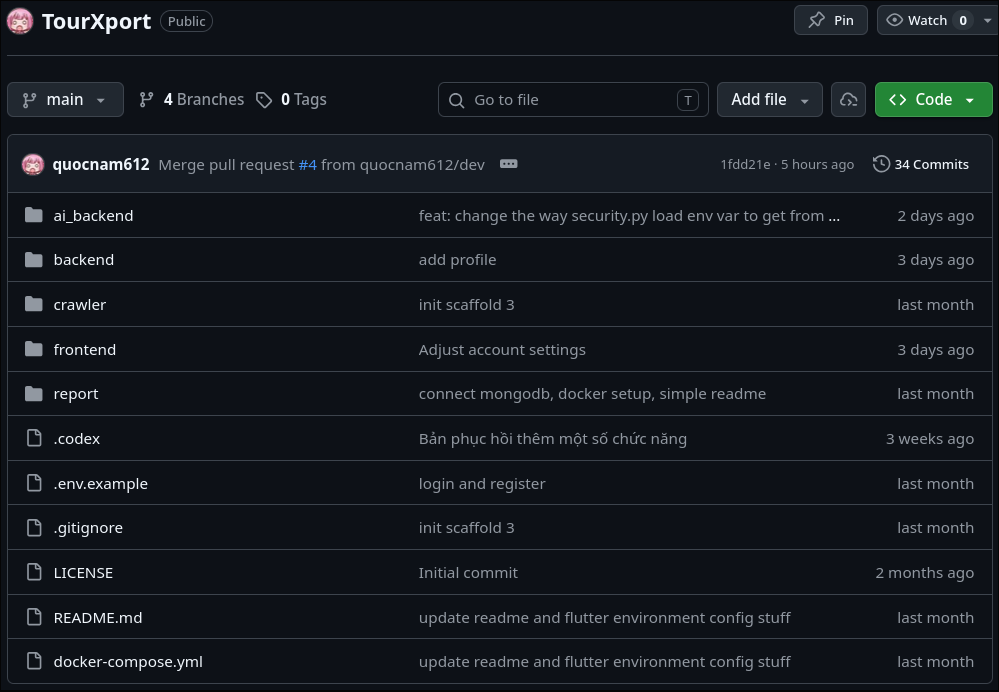
\includegraphics[width=0.6\textwidth]{img/C2-3.png}
    \caption{Kiến trúc thư mục của dự án TourXport}
\end{figure}

\section{Luồng giao tiếp giữa các thành phần}
Luồng dữ liệu trong hệ thống được thực hiện thông qua giao thức HTTP/HTTPS với định dạng dữ liệu chuẩn JSON. Quy trình tương tác điển hình được thực hiện qua các bước sau:

\begin{enumerate}
    \item \textbf{Gửi yêu cầu:} Client gửi yêu cầu kèm theo mã xác thực JWT (JSON Web Token) đến các điểm cuối (endpoints) tương ứng trên Backend Server.
    \item \textbf{Xử lý tại Backend:} Server thực hiện kiểm tra quyền truy cập thông qua các Middleware. Tùy theo loại yêu cầu, server sẽ truy vấn trực tiếp vào cơ sở dữ liệu hoặc gửi tiếp yêu cầu đến dịch vụ AI.
    \item \textbf{Xử lý AI và Dữ liệu:} Dịch vụ AI tiếp nhận yêu cầu, thực hiện truy xuất dữ liệu từ các nguồn đã được chuẩn hóa (Scraped data) để tạo ra phản hồi thông minh.
    \item \textbf{Phản hồi:} Kết quả được đóng gói và trả về Client. Lớp ứng dụng thực hiện giải mã JSON và cập nhật giao diện người dùng ngay lập tức.
\end{enumerate}

\begin{figure}[H]
    \centering
    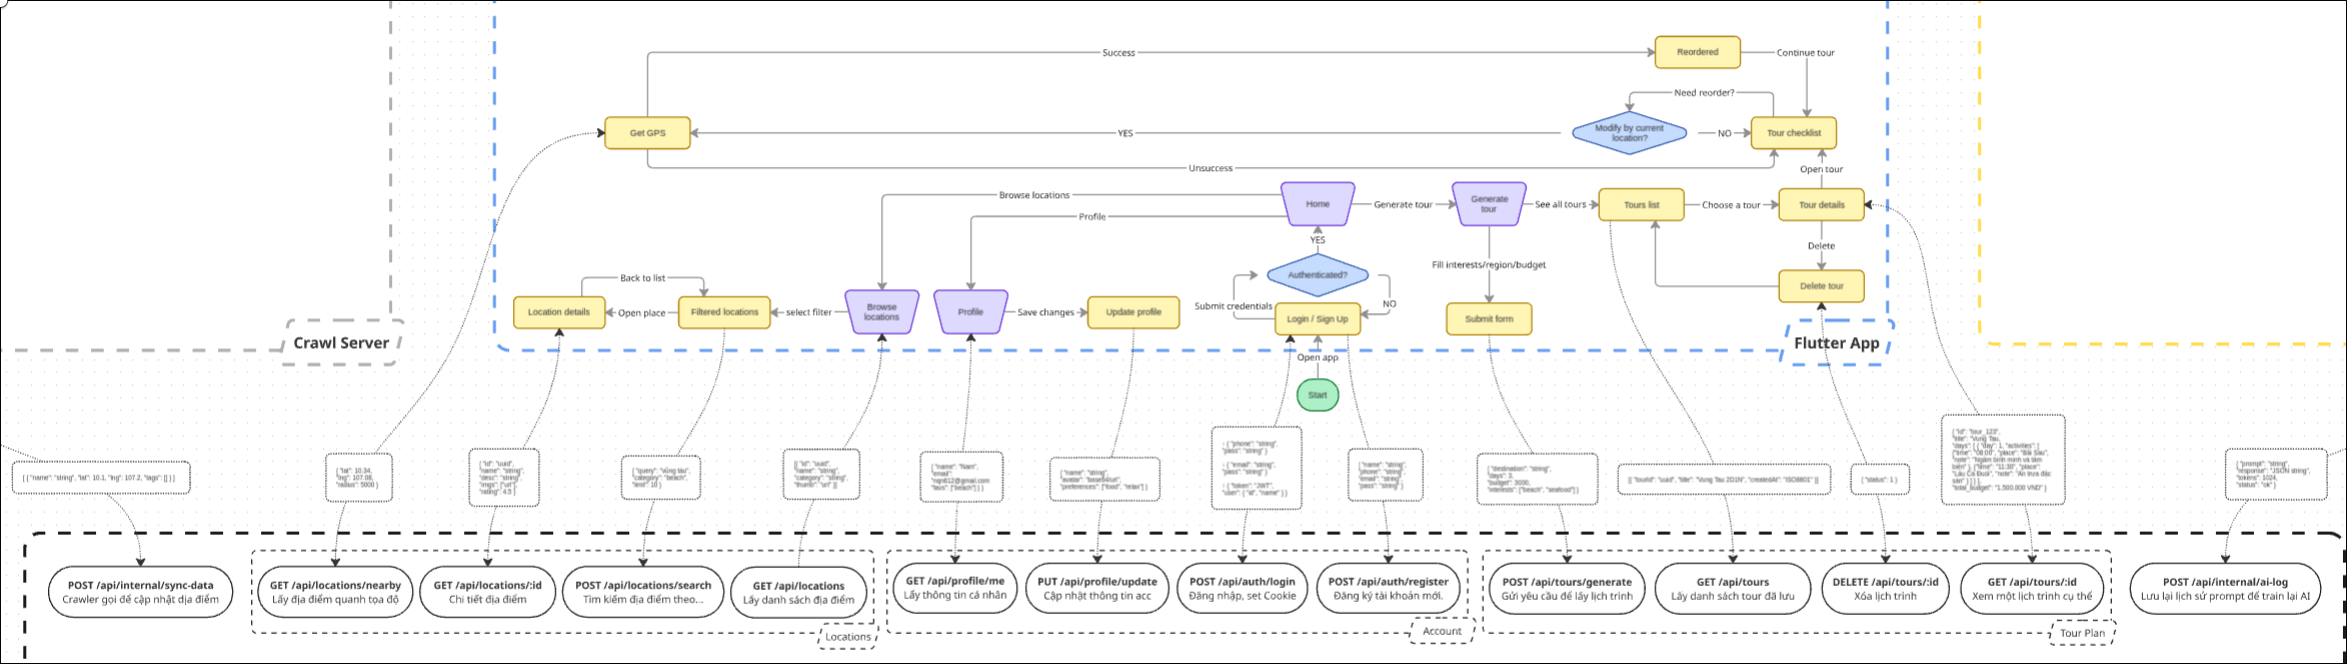
\includegraphics[width=1\textwidth]{img/C2-1.png}
    \caption{Sơ đồ luồng giao tiếp giữa các thành phần của hệ thống TourXport}
\end{figure}

\section{Thiết kế Cơ sở dữ liệu tập trung trên MongoDB}
Cơ sở dữ liệu được thiết kế theo mô hình tập trung, tận dụng khả năng lưu trữ không cấu trúc của MongoDB để tối ưu hóa tốc độ truy xuất. Các thực thể chính bao gồm:

\subsection{Cấu trúc người dùng (User Collection)}
Lưu trữ thông tin định danh, thông tin cá nhân và các cài đặt bảo mật. Mật khẩu được mã hóa trước khi lưu trữ để đảm bảo an toàn dữ liệu.

\subsection{Cấu trúc hành trình (Tour Collection)}
Đây là thành phần cốt lõi của hệ thống, lưu trữ các Tour được tạo ra bởi AI. Cấu trúc bao gồm các mảng lồng nhau (Nested Arrays) để biểu diễn lịch trình theo từng ngày, bao gồm địa điểm, thời gian dự kiến và chi phí ước tính.

\subsection{Cấu trúc địa điểm (Place Collection)}
Chứa dữ liệu đã qua xử lý được thu thập bởi Data Engineer, bao gồm tọa độ địa lý, mô tả chi tiết, hình ảnh và đánh giá chất lượng. Việc tập trung hóa dữ liệu địa điểm giúp giảm độ trễ khi AI thực hiện truy xuất thông tin (RAG).

\begin{figure}[H]
    \centering
    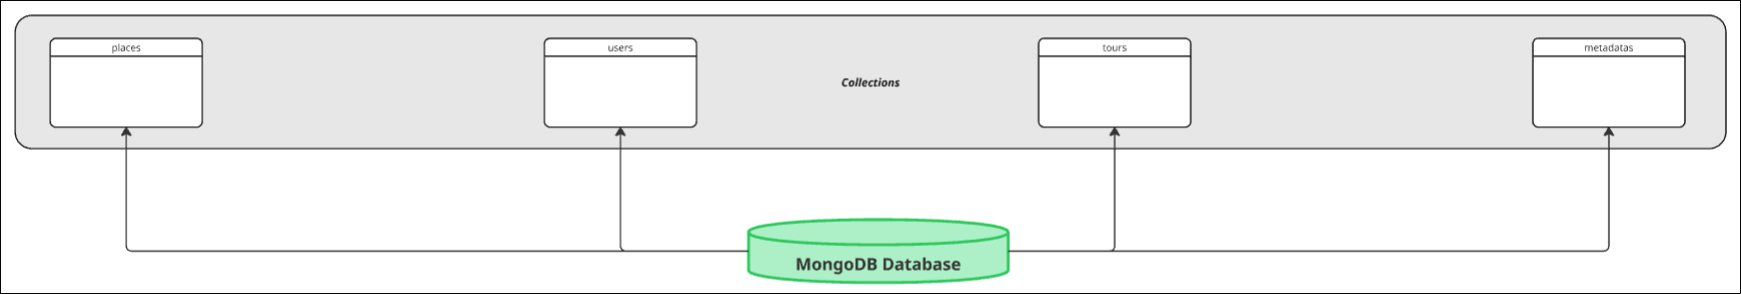
\includegraphics[width=1\textwidth]{img/C2-2.png}
    \caption{Sơ đồ thiết kế cơ sở dữ liệu trên MongoDB}
\end{figure}
\chapter{CHI TIẾT CÁC THÀNH PHẦN CỐT LÕI}

\section{Backend (Node.js \& Express)}
\subsection{Vai trò và Nhiệm vụ}
\subsection{Tech Stack \& Thư viện}
\subsection{Quy trình xử lý}

\section{Frontend (Flutter Multi-platform)}

\subsection{Vai trò và Nhiệm vụ}

\quad Frontend đóng vai trò lớp giao tiếp trực tiếp giữa người dùng và hệ thống TourXport, chịu trách nhiệm xây dựng giao diện, xử lý tương tác và hiển thị dữ liệu một cách trực quan.

\quad Trong dự án TourXport, frontend được phát triển bằng Flutter \cite{fe1} nhằm hỗ trợ đa nền tảng và đảm bảo tính đồng nhất về giao diện trên các thiết bị di động.

\quad Nhiệm vụ chính của frontend trong giai đoạn POC:

\begin{itemize}
    \item Xây dựng Trải nghiệm Người dùng (UX)
    \item Phát triển Giao diện (UI) \cite{fe2}
    \item Thu thập Dữ liệu Người dùng
    \item Xử lý và Hiển thị Dữ liệu
    \item Quản lý Tài khoản
\end{itemize}

\subsection{Tech Stack \& Thư viện}

\quad Front-end của TourXport được xây dựng trên nền tảng công nghệ hiện đại nhằm đảm bảo hiệu năng và tính thẩm mỹ cao:

\begin{itemize}
    \item \textbf{Framework chính}: Flutter cho phép xây dựng ứng dụng đa nền tảng (Android, iOS, Web, Windows) từ một codebase duy nhất.
    \item \textbf{Ngôn ngữ lập trình}: Dart \cite{fe3} là ngôn ngữ tối ưu cho việc xây dựng UI và các tác vụ bất đồng bộ.
    \item \textbf{Thư viện và Công cụ} \cite{fe5}:
        \begin{itemize}
            \item http: Xử lý các yêu cầu mạng (RESTful API) tới Backend.
            \item google\_fonts: Tích hợp bộ font chữ Montserrat chuyên nghiệp
        \end{itemize}
    \item \textbf{Công cụ hỗ trợ}: Figma - thiết kế UI/UX và prototype giao diện
\end{itemize}

\subsection{Quy trình xử lý}

\quad \textbf{Bước 1}: Lên ý tưởng và phân tích yêu cầu
\begin{itemize}
    \item Xác định chức năng cần phát triển
    \item Phân tích nhu cầu người dùng
    \item Xây dựng luồng sử dụng của ứng dụng
\end{itemize}

\quad \textbf{Bước 2}: Thiết kế giao diện trên Figma \cite{fe4}
\begin{itemize}
    \item Chọn màu sắc, font chữ, bố cục
    \item Tạo prototype mô phỏng trải nghiệm người dùng
\end{itemize}

\quad \textbf{Bước 3}: Phát triển giao diện bằng Dart với Flutter
\begin{itemize}
    \item Chuyển thiết kế thành giao diện thực tế
    \item Xây dựng widget và xử lý logic frontend
    \item Kết nối API và quản lý trạng thái ứng dụng
\end{itemize}

\quad \textbf{Bước 4}: Kiểm thử trên máy ảo
\begin{itemize}
    \item Chạy thử trên Android Emulator
    \item Kiểm tra responsive và hiệu năng
    \item Phát hiện và sửa lỗi giao diện/chức năng
\end{itemize}

\subsection{Phân chia công việc}

\subsubsection{Sprint 1}

\begin{figure}[H]
    \centering
    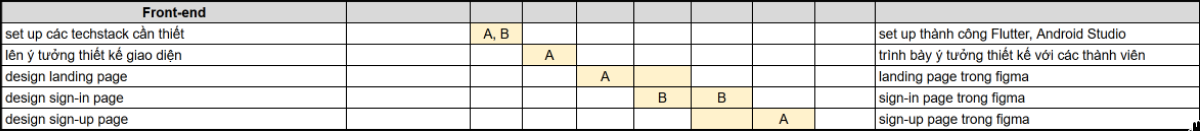
\includegraphics[width=1\textwidth]{img/FEsprint1-1.png}
    \caption{Bảng theo dõi công việc front-end sprint 1}
\end{figure}

\quad Trong Sprint 1, nhóm Front-end tập trung xây dựng nền tảng ban đầu cho ứng dụng bằng Flutter và ngôn ngữ Dart. Mục tiêu chính của sprint là hoàn thành môi trường phát triển, lên ý tưởng giao diện và thiết kế các màn hình cơ bản trên Figma để chuẩn bị cho giai đoạn lập trình.

\quad Các công việc đã thực hiện gồm:
\begin{itemize}
    \item Cài đặt và cấu hình các công nghệ cần thiết như Flutter, Dart và Android Studio.
    \item Thảo luận và thống nhất ý tưởng thiết kế giao diện với các thành viên trong nhóm.
    \item Thiết kế landing page, sign-in page và sign-up page trên Figma.
    \item Xây dựng cấu trúc dự án Flutter ban đầu và kiểm tra khả năng chạy ứng dụng trên máy ảo Android Emulator.
\end{itemize}

\begin{figure}[H]
    \centering
    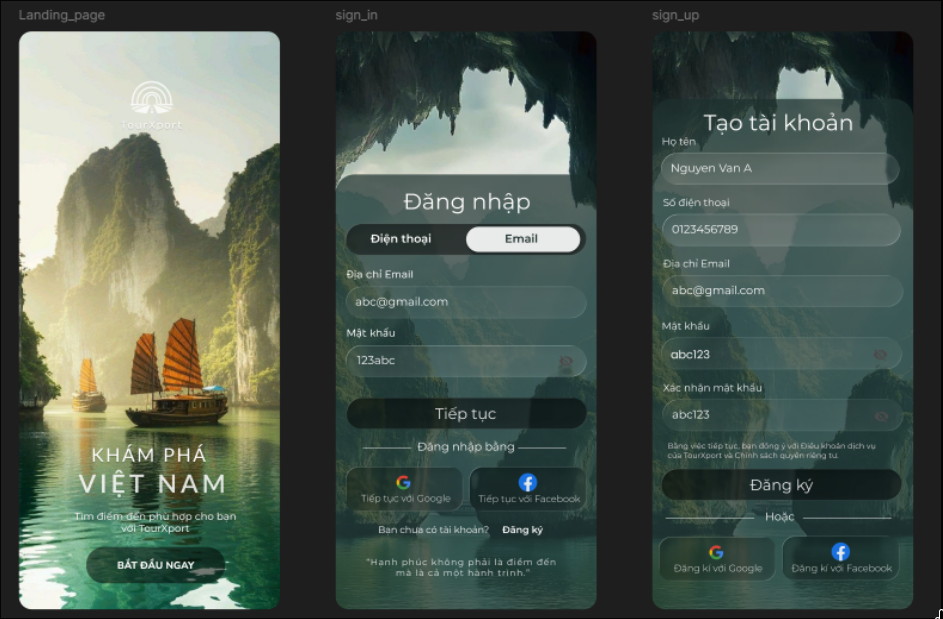
\includegraphics[width=1\textwidth]{img/FEsprint1-2.png}
    \caption{Thiết kế landing page, sign in, sign up}
\end{figure}

\quad Kết quả đạt được sau Sprint 1:
\begin{itemize}
    \item Môi trường phát triển Front-end đã được thiết lập hoàn chỉnh.
    \item Bộ giao diện cơ bản đã được thiết kế thống nhất.
    \item Ứng dụng Flutter có thể khởi chạy và chạy thử nghiệm thành công trên máy ảo.
\end{itemize}

\subsubsection{Sprint 2}

\begin{figure}[H]
    \centering
    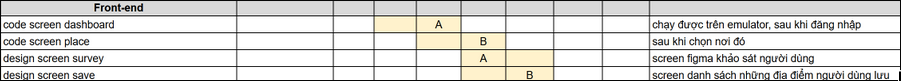
\includegraphics[width=0.9\textwidth]{img/FEsprint2-1.png}
    \caption{Bảng theo dõi công việc front-end sprint 2}
\end{figure}

\quad Trong Sprint 2, nhóm tiếp tục phát triển các chức năng chính của ứng dụng bằng Flutter và Dart. Sprint này tập trung vào việc xây dựng các màn hình chức năng sau khi người dùng đăng nhập, đồng thời mở rộng thiết kế giao diện phục vụ trải nghiệm cá nhân hóa.

\quad Các công việc đã thực hiện gồm:
\begin{itemize}
    \item Phát triển màn hình Dashboard và tích hợp điều hướng cơ bản sau khi đăng nhập.
    \item Xây dựng màn hình Place để hiển thị danh sách địa điểm và chức năng chọn nơi đến.
    \item Thiết kế màn hình Survey nhằm khảo sát sở thích và nhu cầu của người dùng.
    \item Thiết kế màn hình Save để hiển thị danh sách các địa điểm đã được lưu.
\end{itemize}

\begin{figure}[H]
    \centering
    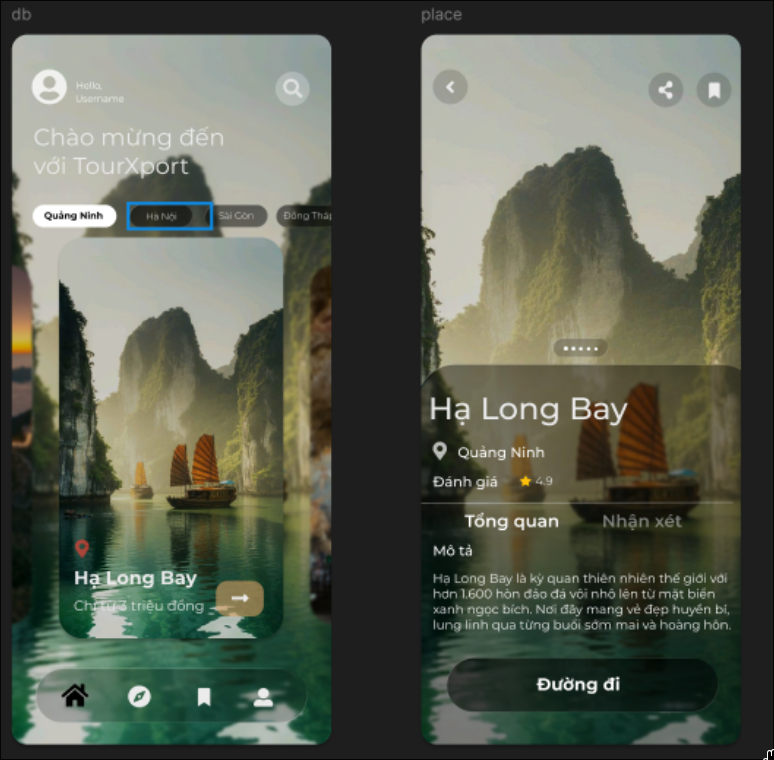
\includegraphics[width=0.6\textwidth]{img/FEsprint2-2.png}
    \caption{Thiết kế dashboard và places}
\end{figure}

\quad Kết quả đạt được sau Sprint 2:
\begin{itemize}
    \item Ứng dụng có thể điều hướng giữa các màn hình chính trên Android Emulator.
    \item Các chức năng giao diện cơ bản sau đăng nhập đã được xây dựng thành công.
    \item Hệ thống giao diện tiếp tục được hoàn thiện và đồng bộ theo thiết kế trên Figma.
\end{itemize}

\subsubsection{Sprint 3}

\begin{figure}[H]
    \centering
    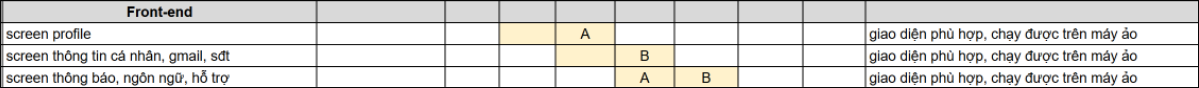
\includegraphics[width=1\textwidth]{img/FEsprint3-1.png}
    \caption{Bảng theo dõi công việc front-end sprint 3}
\end{figure}

\quad Trong Sprint 3, tiếp tục hoàn thiện các chức năng liên quan đến tài khoản và trải nghiệm người dùng bằng Flutter và Dart. Sprint này tập trung phát triển các màn hình cá nhân hóa và cài đặt trong ứng dụng.

\quad Các công việc đã thực hiện gồm:
\begin{itemize}
    \item Xây dựng màn hình Profile với giao diện phù hợp và khả năng hoạt động trên máy ảo.
    \item Phát triển màn hình thông tin cá nhân bao gồm họ tên, Gmail và số điện thoại.
    \item Thiết kế và hoàn thiện màn hình Thông báo, Ngôn ngữ và Hỗ trợ.
    \item Tối ưu bố cục giao diện nhằm đảm bảo tính đồng bộ và thân thiện với người dùng.
\end{itemize}

\begin{figure}[H]
    \centering
    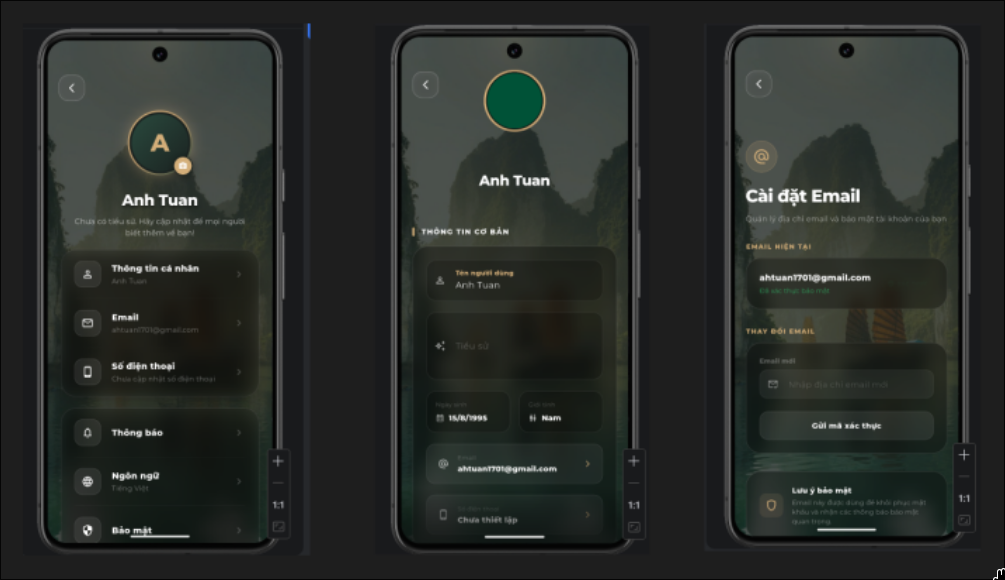
\includegraphics[width=0.9\textwidth]{img/FEsprint3-2.png}
    \caption{Màn hình máy ảo profile và trang thông tin cá nhân, email}
\end{figure}

\quad Kết quả đạt được sau Sprint 3:
\begin{itemize}
    \item Các màn hình quản lý tài khoản và cài đặt đã được xây dựng thành công.
    \item Ứng dụng tiếp tục hoạt động ổn định trên Android Emulator.
    \item Giao diện người dùng được hoàn thiện hơn về tính trực quan và trải nghiệm sử dụng.
\end{itemize}

\section{AI Worker (LLM \& RAG Engine)}
\subsection{Vai trò và Nhiệm vụ}
\subsection{Tech Stack \& Thư viện}
\subsection{Quy trình xử lý}

\section{Thu thập Dataset (Data Crawler/Scraper)}
\subsection{Vai trò và Nhiệm vụ}
\subsection{Tech Stack \& Thư viện}
\subsection{Quy trình xử lý}

\chapter{THỰC THI VÀ ĐÁNH GIÁ THỰC NGHIỆM}

\section{Xây dựng môi trường và triển khai}

\quad TourXport được đóng gói trong các container thông qua công nghệ Docker Compose \cite{docker_compose}, đảm bảo tính nhất quán tuyệt đối về cấu hình môi trường từ máy phát triển cục bộ đến máy chủ thực tế. Tập lệnh docker-compose.yml định nghĩa hạ tầng triển khai song song ba dịch vụ độc lập:

\begin{itemize}
    \item \textbf{Dịch vụ backend}: Triển khai trên môi trường Node.js (Express.js) \cite{nodejs,expressjs} (cổng 3000), thực hiện volume mapping với mã nguồn tại thư mục ./backend và sử dụng công cụ nodemon để tự động nạp lại khi có sự thay đổi mã nguồn.
    
    \item \textbf{Dịch vụ ai\_backend (AI Worker)}: Triển khai môi trường Python 3.10-slim (cổng 8000). Tập lệnh Dockerfile tự động hóa quá trình cài đặt phụ thuộc từ requirements.txt và khởi chạy máy chủ Uvicorn. Dịch vụ này cũng áp dụng cơ chế watch mode để đồng bộ tự động mã nguồn từ thư mục src/ vào bộ chứa. ai\_backend chỉ được expose qua port 8000 nội bộ của Docker, nên chỉ mỗi backend Node.js mới giao tiếp được với ai\_backend.
    
    \item \textbf{Frontend (Flutter)}: Được biên dịch và khởi chạy trực tiếp trên thiết bị thực tế hoặc máy ảo thông qua công cụ dòng lệnh flutter run. Ứng dụng client sẽ giao tiếp với cụm máy chủ thông qua các kiến trúc RESTful API.
\end{itemize}

\section{Kết quả thực thi các Use Case}

\subsection{Use Case Đăng nhập và Xác thực}

\begin{figure}[H]
    \centering
    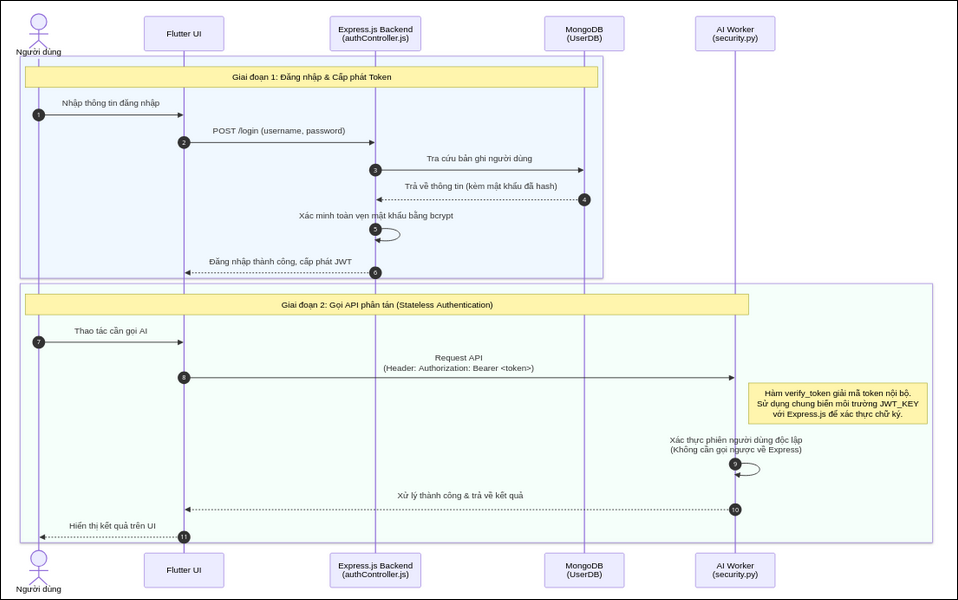
\includegraphics[width=1\textwidth]{img/C4-1.png}
    \caption{Sequence Diagram mô tả use case Đăng nhập và xác thực}
\end{figure}

\quad Khi người dùng gửi thông tin đăng nhập qua giao diện Flutter, Backend Express.js (tại authController.js, hàm login) sẽ tiến hành tra cứu bản ghi trong tập hợp UserDB và xác minh tính toàn vẹn của mật khẩu bằng thuật toán mã hóa bcrypt. Khi đăng nhập thành công, hệ thống cấp phát một JSON Web Token (JWT).

\quad Token này sau đó được gắn vào header của giao thức HTTP (Authorization: Bearer <token>) cho mọi yêu cầu (request) về sau. Điểm đáng chú ý trong kiến trúc phân tán là khi người dùng gọi API của AI Worker, hệ thống AI tự động áp dụng hàm verify\_token (ai\_backend/src/core/security.py) để giải mã token nội bộ. Do AI Worker sử dụng chung một khóa bí mật (biến môi trường JWT\_KEY) với Backend Express.js, nó có thể xác thực được phiên người dùng mà không cần phải gọi API ngược về Backend Express.js, giúp giảm chi phí độ trễ (latency).

\subsection{Use Case Khảo sát nhu cầu người dùng (Survey)}

\quad Trong giai đoạn POC hiện tại, quy trình của Use Case này đang tập trung vào việc xây dựng trải nghiệm thu thập thông tin người dùng ở phía Frontend. Cụ thể, ứng dụng Flutter đã hoàn thiện thiết kế giao diện khảo sát (Survey Screen), cho phép du khách nhập các thông số đầu vào cần thiết cho chuyến đi, bao gồm:

\begin{itemize}
    \item Ngân sách tối đa.
    \item Số ngày dự kiến.
    \item Các sở thích cá nhân cụ thể.
\end{itemize}

\quad Hiện tại, hệ thống đã hoàn tất phần thiết kế UI/UX và các logic quản lý trạng thái biểu mẫu (form state management) trên thiết bị người dùng. Bước tích hợp (Integration) để đóng gói dữ liệu này dưới định dạng JSON và thực hiện lời gọi API thực tế tới endpoint POST /api/trip/generate của AI Worker đang trong lộ trình phát triển và sẽ được hoàn thiện ở các bản cập nhật tiếp theo.

\begin{figure}[H]
    \centering
    \begin{minipage}[t]{0.3\textwidth}
        \centering
        
\includegraphics[width=\textwidth]{img/C4-2.png}
    \end{minipage}
    \hfill
    \begin{minipage}[t]{0.294\textwidth}
        \centering
        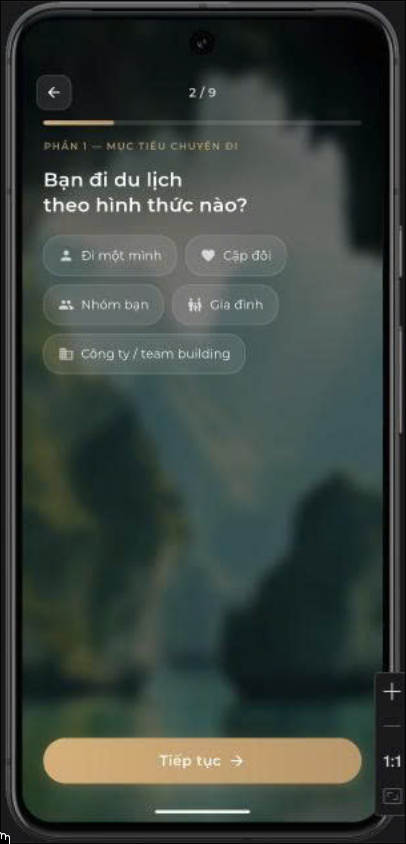
\includegraphics[width=\textwidth]{img/C4-3.png}
    \end{minipage}
    \hfill
    \begin{minipage}[t]{0.29\textwidth}
        \centering
        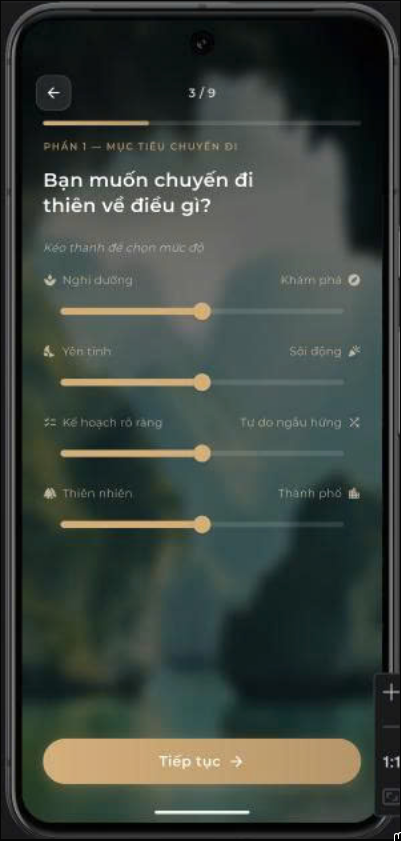
\includegraphics[width=\textwidth]{img/C4-4.png}
    \end{minipage}
    \caption{Màn hình câu hỏi Survey - Mô phỏng trên máy ảo Android}
\end{figure}

\quad Tuy quy trình end-to-end từ Frontend đến Backend chưa được liên kết, toàn bộ luồng xử lý lõi ở phía máy chủ (server-side) đã được xây dựng và kiểm thử độc lập thành công. Khi Frontend sẵn sàng gửi dữ liệu, AI Worker đã có sẵn cơ chế kiểm duyệt dữ liệu tự động thông qua mô hình Pydantic (TripGenerateRequest tại ai\_backend/src/schemas/request/trip\_generator.py). Các request vi phạm điều kiện logic, như ngân sách âm hoặc số ngày vượt quá ngưỡng 30, sẽ bị từ chối ngay lập tức tại cổng API kèm mã lỗi 422 Unprocessable Entity. Khi nhận dữ liệu hợp lệ, luồng Orchestrator sẽ kết nối với OpenAI để sinh ra danh sách các hoạt động du lịch (Location) được phân bổ theo ngày và buổi, tạo tiền đề để Frontend render giao diện timeline sau này.

\begin{figure}[H]
    \centering
    
\includegraphics[width=0.3\textwidth]{img/C4-5.png}
    \caption{Kết quả từ Survey - Mô phỏng trên máy ảo Android}
\end{figure}

\subsection{Đánh giá độ chính xác và hiệu năng hệ thống}

\subsubsection{Hiệu năng hệ thống và độ trễ}

\quad Hệ thống thể hiện hiệu năng tổng thể ổn định và tối ưu xuyên suốt các tầng kiến trúc. Ở phía Client, Frontend Flutter vận hành mượt mà trên đa nền tảng nhờ engine kết xuất đồ họa hiệu năng cao, quản lý trạng thái hiệu quả giúp UI không bị gián đoạn ngay cả khi hiển thị các dữ liệu phức tạp. Tại Server-side, Backend Node.js (Express) xử lý các tác vụ IO chuyên sâu, như truy vấn dữ liệu địa điểm và xác thực người dùng, với độ trễ cực thấp nhờ cơ chế non-blocking I/O.

\quad Đối với hệ thống AI Worker (FastAPI), việc sử dụng hoàn toàn luồng xử lý bất đồng bộ (Asyncio kết hợp thư viện AsyncOpenAI và Motor) giúp giải quyết triệt để nút thắt cổ chai hệ thống. Hiện tại, độ trễ lớn nhất của hệ thống chủ yếu phụ thuộc vào thời gian xử lý tự nhiên của OpenAI API, dao động từ 2 đến 5 giây tùy vào độ dài prompt, trong khi các thành phần nội bộ đều phản hồi gần như tức thời.

\subsubsection{Độ chính xác và tính toàn vẹn dữ liệu}

\quad Dữ liệu của dự án được bảo vệ và kiểm duyệt qua nhiều lớp. Trên Frontend, người dùng bị ràng buộc bởi các form validation, như nhập đúng định dạng email và ngân sách. Khi dữ liệu đến Backend Express, tính toàn vẹn tiếp tục được đảm bảo thông qua hệ thống Mongoose Schema, ví dụ UserDB ép buộc tính duy nhất của email và số điện thoại, bcrypt băm mật khẩu an toàn.

\quad Đối với luồng sinh dữ liệu bằng trí tuệ nhân tạo, hệ thống khắc phục hoàn toàn điểm yếu phổ biến của LLM là trả về JSON bị hỏng (malformed data). Nhờ áp dụng tính năng Structured Outputs của OpenAI kết hợp với cơ chế validate và parse chặt chẽ của Pydantic, tỷ lệ lỗi format kết quả giảm xuống ngưỡng tiệm cận 0%. Các kiểu dữ liệu khó kiểm soát, như số thực float cho chi phí và UUID của địa điểm, luôn được định dạng chính xác tuyệt đối theo API Contract.

\subsubsection{Tính mô-đun và khả năng mở rộng}

\quad Việc thiết kế kiến trúc phân tán (Microservices-oriented) phân tách rạch ròi giữa UI (Flutter), Logic quản trị lõi (Express.js), AI Engine (FastAPI) và Cơ sở dữ liệu tập trung (MongoDB Atlas) mang lại khả năng mở rộng độc lập tuyệt vời. Khi phát sinh trường hợp lưu lượng người dùng yêu cầu sinh lịch trình tăng đột biến, quản trị viên chỉ cần cấp phát thêm tài nguyên riêng cho các container của dịch vụ AI Worker.

\quad Quá trình này diễn ra hoàn toàn biệt lập, không gây ảnh hưởng đến phần lõi quản lý thông tin người dùng hay truy xuất dữ liệu đang vận hành trên cụm Node.js. Song song đó, việc chọn MongoDB làm kho lưu trữ tập trung giúp cả hai backend, Node.js và Python, có thể giao tiếp và truy xuất khối lượng lớn dữ liệu phi cấu trúc một cách linh hoạt, tạo bản lề vững chắc cho việc triển khai các hệ thống phức tạp hơn như RAG (Retrieval-Augmented Generation) trong tương lai.

\chapter{TỔNG KẾT VÀ HƯỚNG PHÁT TRIỂN}

\section{Tổng kết}
\section{Hướng phát triển trong tương lai}


% References
\section{Tài liệu tham khảo}
\nocite{*}
\bibliographystyle{unsrt}
\bibliography{ref/ref}


\end{document}